%%% LaTeX Template: Article/Thesis/etc. with colored headings and special fonts
%%%
%%% Source: http://www.howtotex.com/
% vim: set spell spelllang=es syntax=tex :

\documentclass[12pt]{article}
\usepackage{styles/apuntes-estilo}
\usepackage{fancyhdr,lastpage}
\usepackage{hyperref}
\usepackage[inline]{enumitem}
\usepackage{xurl}
\usepackage{nameref}
\usepackage{tabularx}

\usepackage{appendix}
\renewcommand{\appendixname}{Anexo}
\renewcommand{\appendixtocname}{Anexo}
\renewcommand{\appendixpagename}{Anexo}

\newcommand{\multiline}[2][c]{
      \begin{tabular}[#1]{@{}c@{}}#2\end{tabular}
      }

\def\maketitle{

\makeatletter{
    \color{blue} \centering \huge \sc
    \textbf{
        Trabajo práctico N° 5\\
        \large \vspace*{-8pt} \color{black}
        El software
        \vspace*{8pt}
    }\\
    \small Fecha de finalización: 19 de Junio
    \par
}

\makeatother

\makeatletter
% vim: set spell spelllang=es syntax=tex :
 {\centering \small 
    Introducción a la computación\\
    Departamento de Ingeniería de Computadoras \\
    Facultad de Informática - Universidad Nacional del Comahue \\
    \vspace{20pt} }
\makeatother

\vspace{-2.5cm}
\mbox{\hspace{-1cm}\includegraphics[width=3cm,height=3cm]{logos/uncoma.pdf}\hspace{12cm}
    
\includegraphics[width=3cm,height=3cm]{logos/fai.pdf}}



}

% Custom headers and footers
\fancyhf{} % clear all header and footer fields
\fancypagestyle{plain}{\fancyhf{}}
\pagestyle{fancy}
\lhead{\footnotesize TP N° 5 - El Software}
\rhead{\footnotesize \thepage\ }

\def\ti#1#2{\texttt{#1} & #2 \\ }

\begin{document}

\thispagestyle{empty}
\maketitle
\setlength{\parindent}{1pt}

\textbf{Objetivo:} Comprender la organización y el funcionamiento básico de
una computadora simple. Se involucran conocimientos de los componentes
hardware y sus interacciones para ejecutar instrucciones.

\textbf{Recursos bibliográfico:}

\vspace{-2\topsep}
\begin{itemize}

    \itemsep2pt \parskip0pt \parsep0pt

    \item \emph{Andrew S. Tanenbaum}. Organización de computadoras: un enfoque
        estructurado. Cuarta edición, editorial Pearson Educación, 2000. ISBN
        970-170-399-5.

\end{itemize}

\textbf{Lectura obligatoria:}

\vspace{-2\topsep}
\begin{itemize}

    \itemsep2pt \parskip0pt \parsep0pt

    \item Apuntes de cátedra. Capitulo 5: Arquitectura y Organización de
        Computadoras. Disponible en \textit{PEDCO}:
        \url{https://pedco.uncoma.edu.ar/mod/url/view.php?id=203642}

    \item Apuntes de cátedra. Capitulo 7: El Software. Disponible en
        \textit{PEDCO}:
        \url{https://pedco.uncoma.edu.ar/mod/url/view.php?id=203642}

\end{itemize}

\section{Modelo Computacional Binario Elemental (MCBE)}

\begin{enumerate}

    \item Para los programas que se describen a continuación:

        \begin{enumerate}

            \item Completar la columna de ``Contenido binario'' con la
                codificación en \emph{Lenguaje Máquina} de la instrucción.

            \item Realice una traza del programa e intente identificar que
                tarea realiza el programa. Busque una explicación de alto
                nivel (por ejemplo: \emph{``el programa pide ingresar un número y lo
                multiplica por 3''}, o \emph{``el programa imprime los números del 5
                al 1''}).

            \begin{enumerate}
            \itemsep2em \parskip0pt \parsep0pt

                \item \begin{tabular}{|r||l|l|l||c|}

                    \hline

                    \textbf{\#} & \textbf{Rotulo} & \textbf{Mnemónico/Dato} &
                    \textbf{Argumento} & \textbf{Contenido Binario}\\
                    \hline
                    \hline

                    0 & & LD & IN & 0101 1110\\ \hline
                    1 & & SUB & DATO & \\ \hline
                    2 & & SUB & DATO & \\ \hline
                    3 & & SUB & DATO & \\ \hline
                    4 & & ST & OUT & \\ \hline
                    5 & & HLT & & 0010 0000\\ \hline
                    6 & DATO: & 2 & & 0000 0010\\ \hline

                \end{tabular}

                \item \begin{tabular}{|r||l|l|l||c|}

                    \hline

                    \textbf{\#} & \textbf{Rotulo} & \textbf{Mnemónico/Dato} &
                    \textbf{Argumento} & \textbf{Contenido Binario}\\
                    \hline
                    \hline

                    0 & SALTO2: & LD & DATO & 0100 1001\\ \hline
                    1 & & JZ & SALTO1 & \\ \hline
                    2 & & LD & DATO2 & 0100 1011\\ \hline
                    3 & & ST & OUT & 0111 1111\\ \hline
                    4 & & LD & DATO & \\ \hline
                    5 & & SUB & UNO & \\ \hline
                    6 & & ST & DATO & 0110 1001\\ \hline
                    7 & & JMP & SALTO2 & \\ \hline
                    8 & SALTO1: & HLT & & 0010 0000\\ \hline
                    9 & DATO: & 5 & & 0000 0101\\ \hline
                    10 & UNO: & 1 & & 0000 0001\\ \hline
                    11 & DATO2: & 8 & & 0000 1000\\ \hline

                \end{tabular}

            \end{enumerate}
        \end{enumerate}

    \item Para los programas que se describen a continuación:

        \begin{enumerate}

            \item Completar la columna de ``Mnemónico/Dato'' con la
                codificación en \emph{Lenguaje de Ensamblador} de la
                instrucción o dato.

            \item Realice una traza del programa e intente identificar que
                tarea realiza el programa. Busque una explicación de alto
                nivel (por ejemplo: \emph{``el programa pide ingresar un número y lo
                multiplica por 3''}, o \emph{``el programa imprime los números del 5
                al 1''}).

            \begin{enumerate}
            \itemsep2em \parskip0pt \parsep0pt

                \item \begin{tabular}{|r||c||l|l|l|}

                    \hline

                    \textbf{\#} & \textbf{Contenido Binario} & \textbf{Rotulo}
                    & \textbf{Mnemónico/Dato} & \textbf{Argumento} \\
                    \hline
                    \hline

                    0 & 0101 1110 & & & IN\\ \hline
                    1 & 0110 0110 & & & DATO\\ \hline
                    2 & 0101 1110 & & & IN\\ \hline
                    3 & 1000 0110 & & & DATO\\ \hline
                    4 & 0111 1111 & & & OUT\\ \hline
                    5 & 0010 0000 & & & \\ \hline
                    6 & 0000 0000 & DATO: & & \\ \hline

                \end{tabular}

                \item \begin{tabular}{|r||c||l|l|l|}

                    \hline

                    \textbf{\#} & \textbf{Contenido Binario} & \textbf{Rotulo}
                    & \textbf{Mnemónico/Dato} & \textbf{Argumento} \\
                    \hline
                    \hline

                    0 & 0101 1110 & & & IN\\ \hline
                    1 & 1010 0101 & & & DATO1\\ \hline
                    2 & 0111 1111 & & & OUT\\ \hline
                    3 & 1000 0110 & & & DATO2\\ \hline
                    4 & 0010 0000 & & & \\ \hline
                    5 & 0000 0100 & DATO1: & & \\ \hline
                    6 & 0000 1001 & DATO2: & & \\ \hline

                \end{tabular}

                \item \begin{tabular}{|r||c||l|l|l|}

                    \hline

                    \textbf{\#} & \textbf{Contenido Binario} & \textbf{Rotulo}
                    & \textbf{Mnemónico/Dato} & \textbf{Argumento} \\
                    \hline
                    \hline

                    0 & 0101 1110 & & & IN\\ \hline
                    1 & 0110 1001 & & & DATO\\ \hline
                    2 & 1000 1001 & & & DATO\\ \hline
                    3 & 1000 1001 & & & DATO\\ \hline
                    4 & 1000 1001 & & & DATO\\ \hline
                    5 & 1000 1001 & & & DATO\\ \hline
                    6 & 1010 1010 & & & DATO2\\ \hline
                    7 & 0111 1111 & & & OUT\\ \hline
                    8 & 0010 0000 & & & \\ \hline
                    9 & 0000 0000 & DATO: & & \\ \hline
                    10 & 0000 0011 & DATO2: & & \\ \hline

                \end{tabular}

            \end{enumerate}
        \end{enumerate}

    \item Dado el siguiente programa:

        \begin{tabular}{|r||l|l|l||c|}

            \hline

            \textbf{\#} & \textbf{Rotulo} & \textbf{Mnemónico/Dato} &
            \textbf{Argumento} & \textbf{Contenido Binario} \\
            \hline
            \hline

            0 & & LD & IN & 0101 1110\\ \hline
            1 & SIGUE: & JZ & FIN & 1110 0100\\ \hline
            2 & & ST & OUT & 0111 1111\\ \hline
            3 & & SUB & UNO & 1010 0110\\ \hline
            4 & & JMP & SIGUE & 1101 1101\\ \hline
            5 & FIN: & HLP & & 0010 0000\\ \hline
            6 & UNO: & 1 & & 0000 0001\\ \hline

        \end{tabular}

        \begin{enumerate}

            \item ¿Qué tarea realiza el programa?

            \item ¿Qué modificación seria necesaria realizarle al código
                ensamblador para que el programa imprima cada número dos
                veces? ¿Se modifican la misma cantidad de celdas en el
                programa en código maquina?

        \end{enumerate}

    \item Dado el siguiente programa:

        \begin{tabular}{|r||l|l|l|}

            \hline

            \textbf{\#} & \textbf{Rotulo} & \textbf{Mnemónico/Dato} &
            \textbf{Argumento}\\
            \hline
            \hline

            0 & & LD & IN\\ \hline
            1 & & ST & NUM\\ \hline
            2 & SIGUE: & LD & CANT\\ \hline
            3 & & JZ & IMPRIME\\ \hline
            4 & & SUB & UNO\\ \hline
            5 & & ST & CANT\\ \hline
            6 & & LD & NUM\\ \hline
            7 & & SUB & DOS\\ \hline
            8 & & ST & NUM\\ \hline
            9 & & JMP & SIGUE\\ \hline
            10 & IMPRIME: & LD & NUM\\ \hline
            11 & & ST & OUT\\ \hline
            12 & FIN: & HLT & \\ \hline
            13 & TEST: & -64 & \\ \hline
            14 & NUM: & 0 & \\ \hline
            15 & CANT: & 5 & \\ \hline
            16 & UNO: & 1 & \\ \hline
            17 & DOS: & 2 & \\ \hline

        \end{tabular}

        \begin{enumerate}

            \item ¿Qué tarea realiza el programa?

            \item ¿Cual sera el comportamiento del programa si se cambia la
                instrucción en la dirección nueve por ``\textbf{JMP TEST}''?

        \end{enumerate}


    \item Analice y responda las siguientes preguntas, justificando su
        respuesta:

        \begin{enumerate}

            \item ¿Cuál es la dirección de la primera instrucción que
                ejecutará la máquina?

            \item ¿Cuál es el rango de valores del acumulador del \emph{MCBE}?

            \item ¿A qué distancia máxima puede ``saltar'' el control del
                programa?

            \item ¿Cuál es la dirección más alta donde puede encontrarse una
                instrucción a ser ejecutada?

            \item ¿Puede el \emph{MCBE} encontrar una instrucción que no sea
                capaz de decodificar?

            \item ¿Qué utilidad tendría un programa que no hiciera ningún uso
                de la Unidad de \emph{Entrada/Salida} para comunicar sus
                resultados?

            \item Supongamos que hemos almacenado en la posición 14 un dato
                numérico que representa la edad de una persona. ¿Qué pasa si
                en algún momento de la ejecución el \emph{PC} contiene el
                número 14?  ¿Qué pasará si esa persona tiene 33 años? ¿Qué
                pasará si tiene 65?

            \item ¿Qué pasa si el programa no contiene una instrucción
                \emph{HLT}?

            \item Un programa ¿Puede modificarse a sí mismo? ¿Esto es útil?
                ¿Conveniente? ¿Peligroso?

            \item ¿Podría aumentarse la capacidad de memoria de el
                \emph{MCBE}? ¿Esto requeriría algún cambio adicional a la
                máquina?

            \item ¿Cómo se podría aumentar la cantidad de instrucciones
                diferentes de el \emph{MCBE}? ¿Esto tendría algún efecto sobre
                la longitud de los programas que puede ejecutar la máquina?

            \item Si una nueva arquitectura tiene instrucciones con 5 bits
                para el código de operación y 10 para operando (donde en el
                caso de las instrucciones de carga y almacenamiento indican la
                dirección de la celda origen o destino) ¿Cuantas operaciones
                distintas puede tener como máximo esta arquitectura? ¿Cuantas
                celdas de memoria puede tener?

            \item Se desea establecer el tamaño mínimo para una arquitectura
                que tiene 14 instrucciones distintas, y cada instrucción tiene
                tres operandos, donde cada operando referencia una de las 512
                celdas de memoria ¿Cuál es la cantidad mínima de bits que
                puede tener una instrucción?

        \end{enumerate}


\end{enumerate}

\appendix
\clearpage
\addappheadtotoc
\appendixpage

\section*{Descripción del Modelo Computacional Binario Elemental (MCBE)}

\begin{description}
    \itemsep2pt \parskip0pt \parsep0pt

    \item[Memoria:] consta de 32 posiciones de 8 bits. Las direcciones 0 a 29
        corresponden a direcciones que pueden ser escritas y leídas. La
        dirección 30 es de \textbf{sólo lectura}, permite leer datos del
        dispositivo de entrada, por ejemplo un teclado. La dirección 31 es de
        \textbf{sólo escritura}, permite escribir datos en el dispositivo de
        salida, por ejemplo en una pantalla o una impresora.

    \item[Registro PC:] registro de 8 bits, contiene la dirección de la
        próxima instrucción a ejecutar. Se inicializa en cero.

    \item[Registro IR:] registro 8 bits donde se guarda la instrucción que se
        esta decodificando o ejecutando.

    \item[Registro acumulador:] registro de 8 bits donde se almacena un
        número entero representado en \emph{complemento a 2}.

    \item[Etiquetas predefinidas:]~

        \begin{description}
            \itemsep2pt \parskip0pt \parsep0pt

            \item[IN:] dirección 30, entrada, dirección de solo lectura.

            \item[OUT:] dirección 31, salida, dirección de solo escritura.

        \end{description}

    \item[Instrucciones:] de 8 bits, los 3 bits más significativos almacenan
        el código de operación, y los 5 menos significativos almacenan el
        operando.

        \begin{figure}[h]
            \centering
            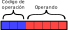
\includegraphics[height=4em]{img/instruccion.pdf}
        \end{figure}

\end{description}

\begin{tabularx}{\textwidth}{c|c|c|X}

    \textbf{Mnemónico/Dato} & \textbf{Código de} & \textbf{Operando} &
    \multicolumn{1}{c}{\textbf{Descripción}} \\

    & \textbf{operación} & & \\

    & \emph{3 bits} & \emph{5 bits} & \\
    \hline
    \hline

    \texttt{LD} & 010 & \emph{dirección} & \textbf{Memoria → Acumulador}. Copia
    un byte desde la dirección de memoria al acumulador. \\ \hline

    \texttt{ST} & 011 & \emph{dirección} & \textbf{Acumulador → Memoria}. Copia
    el contenido del acumulador en esa dirección de memoria. \\ \hline

    \texttt{ADD} & 100 & \emph{dirección} & \textbf{Suma}. El contenido de la
    dirección se suma al acumulador, y el resultado se almacena en el
    acumulador. \\ \hline

    \texttt{SUB} & 101 & \emph{dirección} & \textbf{Resta}. El contenido de la
    dirección se resta al acumulador, y el resultado se almacena en el
    acumulador. \\ \hline

    \texttt{JMP} & 110 & \emph{desplazamiento} & \textbf{Salto incondicional}. Se
    suma (en complemento a 2) el desplazamiento al \textbf{PC}. \\ \hline

    \texttt{JZ} & 111 & \emph{desplazamiento} & \textbf{Salto condicional}. Si
    el acumulador es cero, se suma (en complemento a 2) el desplazamiento al
    \textbf{PC}, en caso contrario el \textbf{PC} se incrementa en uno. \\
    \hline

    \texttt{HLT} & 001 & \emph{(sin uso)} & \textbf{Detiene la maquina}. No se
    ejecutan nuevas instrucciones. Los registros y la memoria quedan con el
    último valor que tenían. \\ \hline

    \texttt{NOP} & 000 & \emph{(sin uso)} & \textbf{No operación}. No tiene
    ningún efecto sobre el acumulador ni memoria. El \textbf{PC} se incremente
    en uno. \\

\end{tabularx}

\end{document}
